\documentclass[12pt] {article}
\usepackage{times}
\usepackage[margin=0.6in,bottom=1in,top=0.9in]{geometry}

\usepackage{hhline}
\usepackage{subfig}
\usepackage{graphicx}
\usepackage{amsmath}




\begin{document}

\title{Final Project - Load Balancing on Graph Coloring}
\author{Yuxin Chen and Ruolan Zeng}
\date{March 22nd, 2018}
\maketitle
%============Table========
%\begin{figure}[tbh]
% \centering    
%\begin{tabular}{ |p{4cm}|| p{2cm}|p{2cm}|p{2cm}|p{2cm}|}
% \hline
% & Processor 1 &  Processor 2  & Processor 3 & Processor 4\\ \hhline{|=|=|=|=|=|}
% \hline
% Performance          &$1.08$        &$1.425$       &\textbf{1.52}  &   \\
% \hline
%\end{tabular} 
%\caption{Metric table for the four processors}
%   \label{tab:metric}
%\end{figure} 
%============Figure========
%\begin{figure}[!tbh]
%\centering        
%   \subfloat {\includegraphics[width=0.65\textwidth]{fig2_4.png}}
%   \caption{ }
%   \label{fig:fig}
%\end{figure}

\section*{Algorithm Details:}
There are two approaches to do graph coloring: 1) independent set (IDS) based 2) greedy algorithm based. In our work, we chose to use the independent set based algorithm. %Basically we generate a random number for each node; then a node can be added to the current independent set only if it has the maximum random number among its neighbors. This method ensures every node within the same independent set to be colored; they are not connected. Next iteration we find the maximum vertex on nodes left (exclude nodes which are in the independent sets) and form a new independent set. The algorithm continues until all the nodes belong to independent sets.
The IDS-based algorithm first assigns a random number for each node in the input graph. Then the algorithm proceeds by adding the nodes with maximum random number among their neighbor (nodes they are connected to) to an independent set. Nodes in an independent set are colored with the same colors and deleted from the graph. The process continues between two phases; finding IDS and coloring the IDS and deleting it from the graph until all nodes are colored. 

\section*{An naive implementation}
A naive implementation: 
We map each thread to each node, and each thread will look up all the node's neighbors and see if the node is the maximum among its neighbors. If yes, assign the current
color to the node.

There might be some load balancing problem. Some nodes might have a lot of neighbors, and some might have few. Then the threads mapped to the nodes with longer neighbor
list keep busy while the threads mapped to the nodes with short neighbor list stay idle. This will hurt the performance badly. The GPU resource is not fully
utilized.

\section*{Use three Kernels to achieve load balancing}
As we explained before, the performance might hurt because of the big variance of neighbor list length. Then we would like to process the nodes with huge neighbor list first
with a block of threads. Then we process the nodes with the medium neighbor list with a warp of threads. Last we process the nodes with the small neighbor list with just threads.

In this way, we could expect to get a better load balancing, thought strickly speaking, the kernel which processes the huge neighbor list might still kind of imbalanced. To
do so, we need to group the nodes according to their degree. Here, we sacrifice memory for better performance by writing three predicate array for nodes which has
degree larger than 512, larger than 32 and less than 512 and less than 32 respectively. Then we can scan on those three predicate arrays and copy the nodes to large
degree array, medium degree array, and small degree array according to their degree. As the figure ~ \ref{fig:fig1} shows.

\begin{figure}[!tbh]
\centering        
   \subfloat {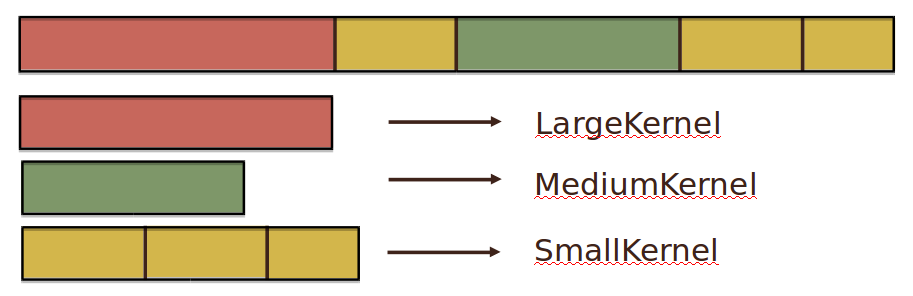
\includegraphics[width=0.65\textwidth]{threekernel.png}}
   \caption{ three kernels load balancing }
   \label{fig:fig1}
\end{figure}

Then I call LargeKernel which I assign a thread block to process a node on large degree array, call MediumKernel which I assign a wrap to process a node in medium degree
array, and call SmallKernel which I assign a thread to process a node with small degree. How to decide the threshold of large degree, medium degree, and small degree is
little heuristic. We use 512, 32 respectively in our experiments. 

\section*{Using load balancing Search to achieve load balancing }

The key point for this approach is that each thread will get the same amount of elements for CSR's col\_id array like the figure  ~ \ref{fig:fig2} illustrates. The task of algorithm requires each element in the CSR's col\_id array to compare its random number with its owner's random number. Then each thread mapped to each element need to know who is its owner. The function: load\_balance\_search will give an array which is the same size of col\_id, to tell who is the owner of the corresponding element in the col\_id. 

\begin{figure}[!tbh]
\centering        
   \subfloat {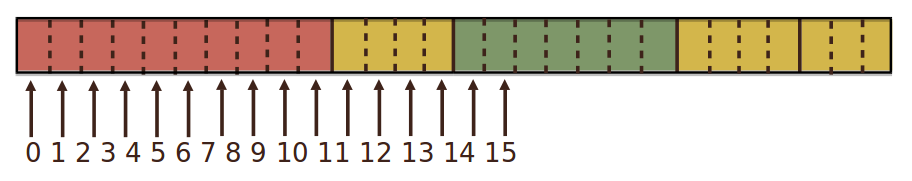
\includegraphics[width=0.64\textwidth]{lbs.png}}
   \caption{ load balancing search load balancing }
   \label{fig:fig2}
\end{figure}

Using this approach, even the variance of neighbor list length of each node is very high; tasks are evenly distributed among threads. Thus the computation is more load balanced.
\\\\\\\\\\\\\\\\\\\\\\\\\\\\\\\\\\\\\
\section*{Numerical Experiments:}
Here we show some results of our implementation. Table ~\ref{tab:results1} shows some features of the graphs we use in our experiments. So myciel and planar43264 are both sparse graph with max degree less than 32. myciel is very small, and planar43264 is larger. gq.order100 is a medium dense graph, and dsjc1000 is a very dense graph. len450 has some variance on the degree of nodes, ranging from 29 to 68. Table ~ \ref{tab:results2} shows the results and comparison among naive implementation and implementation using three kernels and load balancing search. We found that usually load balancing search works pretty well in all kind of graphs. Three kernel approach works pretty well in high variance degree graph and dense graph. There is a dataset which naive implementation won. This also makes sense. The Planar graph has the max degree of the node of 4. Otherwise, it cannot be planar. Planner graph itself is very load balanced, using load balancing techniques only add overhead since they are not free. 

\begin{figure}[tbh]
 \centering    
\begin{tabular}{ |p{2.9cm}||p{1.7cm}| p{1.7cm}|p{1.7cm}|p{2.2cm}|p{3cm}|p{2.4cm}|}
 \hline
   & $\#$Vertices & Edges &  Average Degree & Vertices (Degree$<$32) & Vertices (32$\leq$Degree$<$512) &Vertices (Degree$>$512) \\ 
     
     \hhline{|=||=|=|=|=|=|=|}
 \hline
 le450\_5d.col &450       & 9757  & 43.36 &21  &429 & 0\\
 \hline
 myciel4.col &  23       & 71  &3.08  &23  &0  &0\\
 \hline
   planar43264.col & 43264     &  259524 & 5.998  &43264 & 0 &0 \\
 \hline
   qg.order100.col &10000  &990000  & 99  & 0 & 10000 & 0 \\
 \hline
   dsjc1000.9.col & 1000  & 449449 & 449.44  & 0 & 0 & 1000 \\
 \hline
 \hline
 
 
\end{tabular} 
\caption{Sumarry of datasets}
   \label{tab:results1}
\end{figure} 

\begin{figure}[tbh]
 \centering    
\begin{tabular}{ |p{4cm}||p{3cm}|| p{4cm}|p{4cm}|}
 \hline
   & $\#$Naive & Three Kernels &  Load Balancing Search \\ 
     
     \hhline{|=||=|=|=|}
 \hline
 le450\_5d.col & 4.4231ms  & 2.990ms  &657.198us \\
 \hline
 myciel4.col & 69.378us       & 133.122us  &65.571us \\
 \hline
   planar43264.col & 416.01us &  107.00ms & 848.125us\\
 \hline
   qg.order100.col & 54.098ms & 36.883ms   & 34.17ms\\
 \hline
   dsjc1000.9.col & 850.73ms & 48.176ms   &46.57ms \\
 \hline
 
 
\end{tabular} 
\caption{Results and comparison of our implementation using different load balancing techniques.}
   \label{tab:results2}
\end{figure} 


\end{document}
